\chapter{Módulo de explicação}
\label{cap:explicacao}

As explicações assentam num princípio: a justificação de cada conclusão é
registada no momento da inferência, e não reconstruída depois. É a ideia que
se manteve do motor da unidade curricular (\cref{sec:comparacao-motor-uc}),
aplicada a dois níveis. No motor Prolog, cada facto guarda
como foi obtido. Na aplicação, cada ciclo de decisão guarda as propostas das
regras e o resultado da arbitragem.

\section{O que fica registado}
\label{sec:expl-registo}

Em cada ciclo, o motor Prolog regista:

\begin{itemize}
  \item para cada facto derivado, \texttt{wm\_support(Id, Regra, Evidência)}: a
    regra que o concluiu, os factos em que assentou e os padrões negados que se
    verificaram;
  \item para cada proposta, a ação, a velocidade, o risco, a prioridade, a
    razão, a regra e a evidência. A evidência é a lista desses factos, e cada
    facto derivado indica a regra que o concluiu, por exemplo
    \cod{pedestrian_conflict(p1) (by rule '...')};
  \item os quatro subobjetivos de \cod{safe_to_change_lane/1}
    (\cod{maneuver_idle}, \cod{no_continuous_line}, \cod{side_clear},
    \cod{room_to_follow}), provados um a um nos dois lados por
    \cod{subgoal_results/2}, mesmo quando nenhuma regra propõe mudar de via;
  \item uma entrada na linha temporal por cada leitura dos sensores
    (\cod{FACT INSERTED}) e por cada regra que concluiu algo
    (\cod{RULE FIRED}).
\end{itemize}

A camada Java junta a cada proposta o seu resultado na arbitragem: venceu,
perdeu para outra, foi vetada por uma paragem obrigatória, foi limitada por um
teto de velocidade, ou foi recusada pelo atuador. Junta também um detalhe que
identifica a regra vencedora ou o motivo da recusa.

\begin{figure}[H]
  \centering
  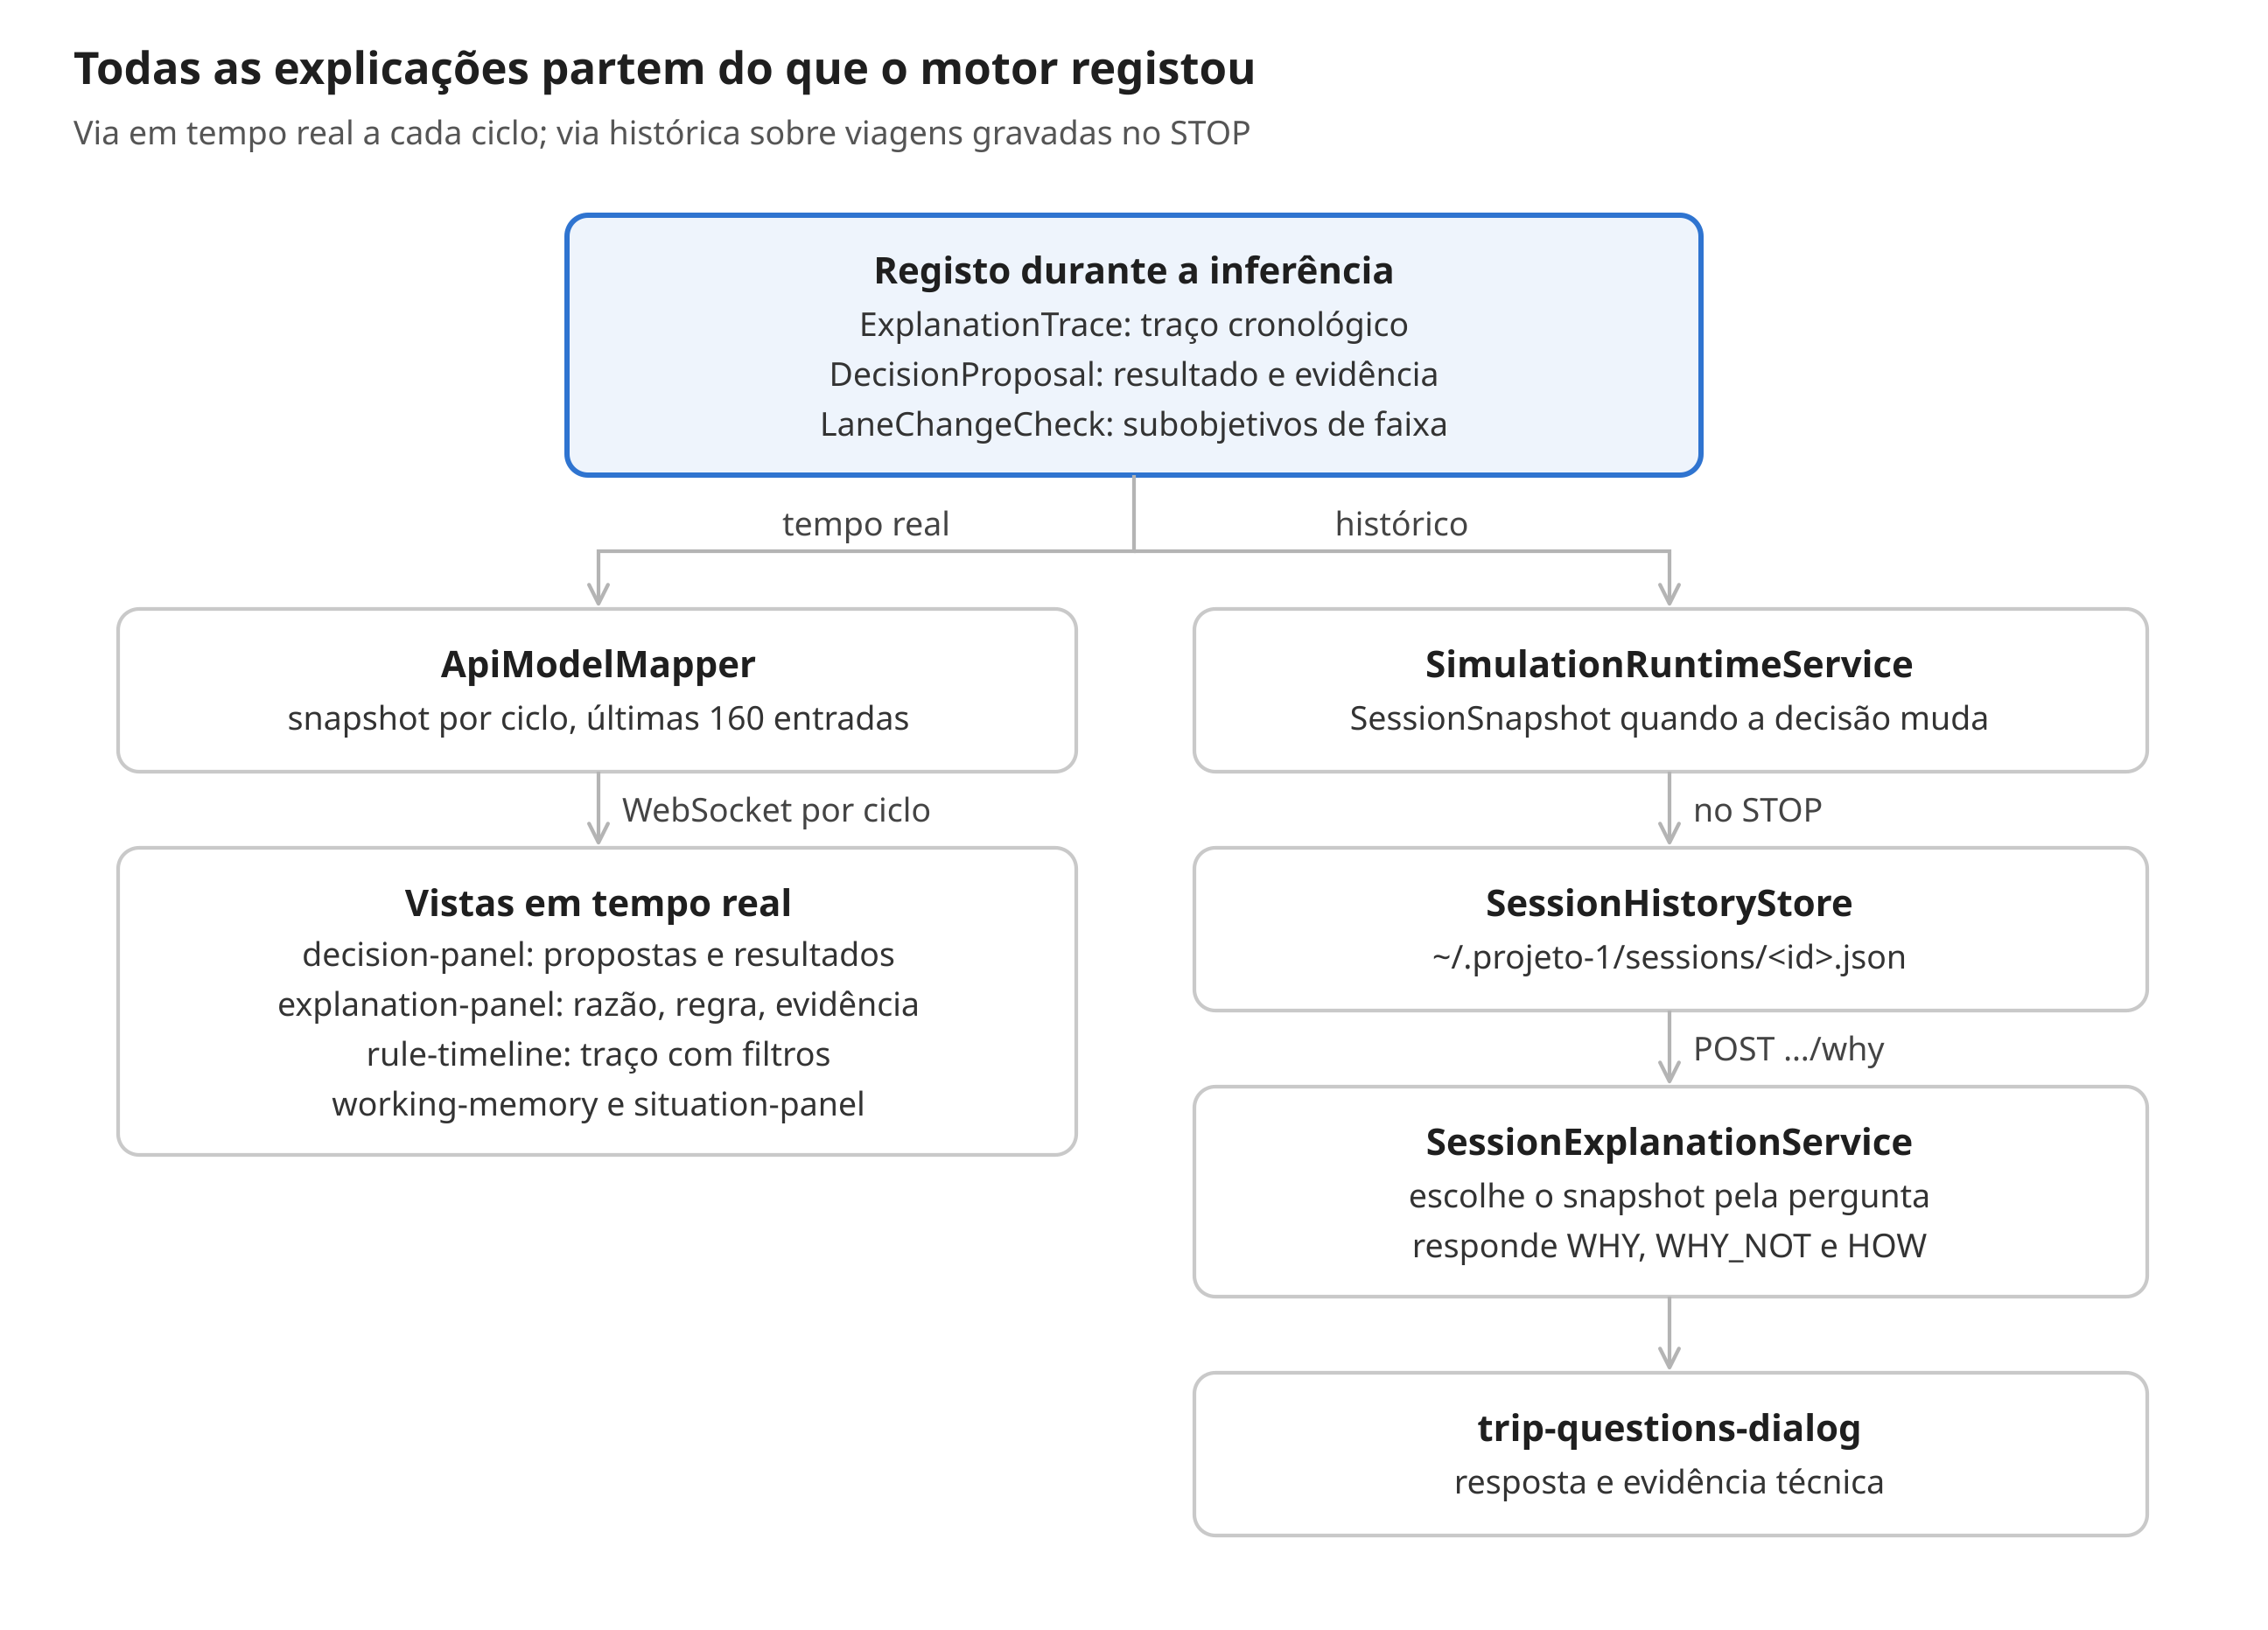
\includegraphics[width=0.70\textwidth]{figuras/explicacao-duas-vias.png}
  \caption{Percurso da informação no módulo de explicação: o percurso em tempo real, a cada ciclo, e o percurso histórico, sobre a viagem gravada ao parar.}
  \label{fig:explicacao-duas-vias}
\end{figure}

Os dois percursos da \cref{fig:explicacao-duas-vias} partem do mesmo registo. No
percurso em tempo real, o estado de cada ciclo chega à interface pelo WebSocket. O painel
de decisão mostra cada proposta com o seu resultado na arbitragem, e outros
painéis mostram a razão, a regra, a evidência, a linha temporal e a memória de
trabalho. No percurso histórico, guarda-se um registo completo do ciclo
(\cod{SessionSnapshot}) sempre que a decisão muda. Quando o utilizador carrega
no botão \enquote{STOP} da interface Web, abre-se um
diálogo em que pode percorrer as decisões registadas. Para cada uma, a interface
permite consultar os três tipos de explicação, \emph{How}, \emph{Why} e
\emph{Why not} (ver também a \cref{sec:interface}).

\paragraph{Exemplo.} Nas secções seguintes usa-se a mesma situação, executada no
motor Prolog. O veículo segue a 50\,km/h na via da direita, há um buraco na
mesma via 40\,m à frente, e a via da esquerda está livre. A regra
\cod{'Avoid pothole in right lane by changing left'} (prioridade 40) propõe
\cod{CHANGE_LANE_LEFT}, e a regra de base mantém a velocidade.

\section{How}
\label{sec:expl-how}

No motor, \cod{explain/2} percorre as justificações \cod{wm_support/3}
recursivamente e devolve a árvore de derivação como um termo. Cada facto
derivado é um nó \cod{derived(Facto, Regra, Porque)}, cada facto percebido é uma
folha \cod{perceived(Facto)}, e cada padrão negado é \texttt{absent(Padrão)}. A
\cref{lst:arvore-how} mostra a árvore da proposta do exemplo.

\begin{lstlisting}[caption={Árvore de derivação devolvida por \texttt{explain/2} para a proposta do exemplo},label=lst:arvore-how]
derived(proposal(change_lane_left, no_target, low, road_hazard,
                 'Avoiding pothole by moving into the clear left lane'),
        'Avoid pothole in right lane by changing left',
        [ perceived(ego_lane(right)),       perceived(pothole(p1,40,high,right)),
          perceived(ego_speed(50)),         perceived(lane_change_state(idle)),
          perceived(right_marking(dashed)), perceived(lane_occupancy(left,false,inf)) ])
\end{lstlisting}

A árvore tem seis factos, embora as condições da regra só nomeiem três
(\cod{ego_lane}, \cod{pothole} e \cod{ego_speed}). Os outros três vêm da prova de
\cod{safe_to_change_lane(left)}, feita por \emph{backward chaining}
(\cod{prove/1}): a prova regista os factos que lê com \cod{known/1}, e estes
passam a fazer parte da evidência. Quando a decisão depende de conclusões
intermédias, como \cod{pedestrian_conflict/1}, a árvore desce por elas.

Para obter esta árvore, optou-se por não usar o rastreio do SWI-Prolog
(\cod{trace/0}). O rastreio mostra a resolução feita pelo próprio interpretador,
com as chamadas, saídas, retrocessos e falhas de cada predicado, incluindo os do
motor (\cod{findall/3}, \cod{msort/2}), e não as regras de condução que
dispararam nem os factos em que assentaram. Além disso, é interativo e obriga
a executar em modo de depuração, mais lento. Como o motor trata as
próprias regras como dados, é ele que regista, no momento de cada disparo, a
regra e a evidência (\cod{wm_support/3}), e é desse registo que \cod{explain/2}
constrói a árvore.

Na aplicação, o \emph{How} mostra o caminho que o ciclo escolhido percorreu no
fluxograma de decisão da velocidade e no da via. Cada pergunta do fluxograma
segue o ramo \enquote{sim} quando uma das regras que lhe respondem fez uma
proposta nesse ciclo, e o caminho termina onde a arbitragem fixou a decisão.

\section{Why}
\label{sec:expl-why}

Nos materiais da unidade curricular, o \emph{Why} é o do MYCIN: quando o motor
pergunta um facto ao utilizador, este pode perguntar porquê, e o motor mostra a
regra que está a tentar provar (o \cod{sp_exp2.pl} não o
implementa). Este
sistema não faz perguntas ao utilizador. Todos os factos vêm dos sensores e do
estado do veículo, dez vezes por segundo, um ritmo a que nenhum condutor
conseguiria responder. Por isso, aqui, o \emph{Why} justifica uma decisão já
tomada: responde porque é que o veículo fez o que fez. Para cada canal, a
aplicação junta a regra que decidiu, a sua razão, a evidência e o resultado da
arbitragem, bem como as outras propostas que também foram consideradas. No canal
da via, uma mudança de via inclui ainda os subobjetivos de segurança desse
lado. No exemplo, o veículo muda para a esquerda porque
\cod{'Avoid pothole in right lane by changing left'} se verificou, com a razão
\enquote{Avoiding pothole by moving into the clear left lane}. A evidência são
os seis factos acima, e os quatro subobjetivos de
\cod{safe_to_change_lane(left)} verificaram-se. A velocidade mantém-se porque
nenhuma regra encontrou motivo para acelerar ou abrandar.

\section{Why not}
\label{sec:expl-whynot}

O \emph{Why not} responde porque é que o veículo não fez outra coisa. Na
interface, o utilizador pergunta por uma alternativa, por exemplo
\enquote{porque não abrandou para o buraco?}, e a resposta vem de dois
mecanismos. Um terceiro, no motor, desce até à condição exata de uma regra:

\begin{itemize}
  \item \textbf{Uma alternativa não escolhida.} Para cada alternativa que o
    ciclo não seguiu, na velocidade ou na via, a aplicação explica porquê, a
    partir do registo do ciclo. Ou foi proposta mas perdeu na arbitragem (e a resposta diz
    para que regra, e por que princípio), ou nunca foi proposta porque as suas
    condições não se verificaram, ou não se aplica naquele estado, ou o ciclo
    não registou o suficiente. No último caso, a resposta di-lo em vez de
    adivinhar. No exemplo, \enquote{porque não abrandou?} tem como resposta que
    nenhuma regra encontrou uma condição que exigisse abrandar, e
    \enquote{porque não mudou para a direita?} não se aplica, porque o veículo
    já está na via mais à direita.
  \item \textbf{Uma mudança de via recusada.} Os subobjetivos de
    \cod{safe_to_change_lane/1} registados em cada ciclo dizem qual deles
    falhou. Em vez de uma mensagem genérica como \enquote{mudança impossível}, a
    explicação indica a causa: outra manobra em curso, linha contínua, ângulo
    morto ocupado, ou falta de distância para seguir o veículo da outra via.
  \item \textbf{Uma regra que não disparou.} No motor, \cod{why_not/2} procura,
    entre todas as correspondências parciais das condições da regra, da esquerda
    para a direita, a que avançou mais. Devolve a condição onde parou, com as
    ligações dessa correspondência, seguida das condições posteriores que também
    falham. Chega-se a ele pelo pedido \cod{whynot} do \cod{server.pl}. No
    exemplo, para a regra que abranda perante um buraco, aponta a condição
    negada que falhou: o buraco ainda pode ser contornado (\cref{lst:whynot}).
\end{itemize}

\begin{lstlisting}[language=JSON,caption={Pedido \texttt{whynot} e resposta do \texttt{server.pl} no exemplo},label=lst:whynot]
{"cmd":"whynot", "rule":"Pothole ahead reduce speed"}
{"ok":true, "rule":"Pothole ahead reduce speed",
 "failedConditions":["not(test(pothole_avoidable_now(50,40)))"]}
\end{lstlisting}
